This section describes the purpose, use, and intended user audience for the RV8 Work Cell. RV8 Work Cell is a system that performs palletizing and depalletizing of boxes in an industrial manner. Users of this work cell will be able to practice standards in industrial robotics, while increasing time efficiency. 
\subsection{Purpose and Use}
The conventional approach to material handling in warehouses contains several challenges. Palletizing and depalletizing boxes manually is a time-consuming task, which decreases productivity. Moreover, manual material handling poses inherent risks to the workforce. Accidents and injuries are a constant concern, impacting both employee well-being and company reputation. Finally, with modern commerce continuing to grow, warehouses must adapt to higher volumes of goods and fulfill needs with efficiency. Manual processes often hinder the ability to meet customer demands effectively. The RV8 robot work cell will palletize and depalletize boxes in an organized manner according to customer's requirements with high efficiency and accuracy.

\subsection{Intended Audience}
This product is considered industrial, so the intended audience of this product are warehouses and factories where manual labor can be automated through the use of robotics.

\begin{figure}[h!]
	\centering
   	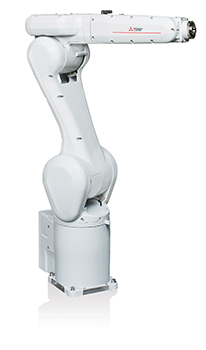
\includegraphics[width=0.40\textwidth]{images/rv8crl.jpeg}
    \caption{Mitsubishi RV8-CRL  \cite{MitsubishiRV8CRL}}
\end{figure}
